\subsection*{Punto 01}

\textbf{Genere un conjunto de datos de entrenamiento de 200 puntos en $\mathcal{R}^3$ muestreando 100 puntos con coordendas independientes de una normal $\mathcal{N}(4,1)$ y 100 puntos de una normal $\mathcal{N}(8,1)$. Ejecute el algoritmo de agrupamiento de k-medias, para k = 2, 3,..., 15, usando el conjunto de datos de entrenamiento. Para cada k use diez puntos iniciales aleatorios y solo guarde la solución que tenga el menor valor de la función objetivo de k-medias. Muestra en una gráfica el valor de la función objetivo de k-medias resultante sobre el conjunto de datos de entrenamiento como una función de k. Comenta lo que ves. Qué valor de k seleccionaría basándose solo en esta gráfica?}

En la figura \ref{fig:problema_03_train_scores} se muestran los resultados de la función objetivo objetivos con el número de clusters $k=2,3,\dots,15$. En esta gráfica se observa el comportamiento descendiente de la función objetivo conforme aumentan el número de clusters a tomar en cuenta. Este comportamiento aparenta llegar a una convergencia a un valor fijo conforme el número de clusters aumenta.

\begin{figure}[H]
    \centering
    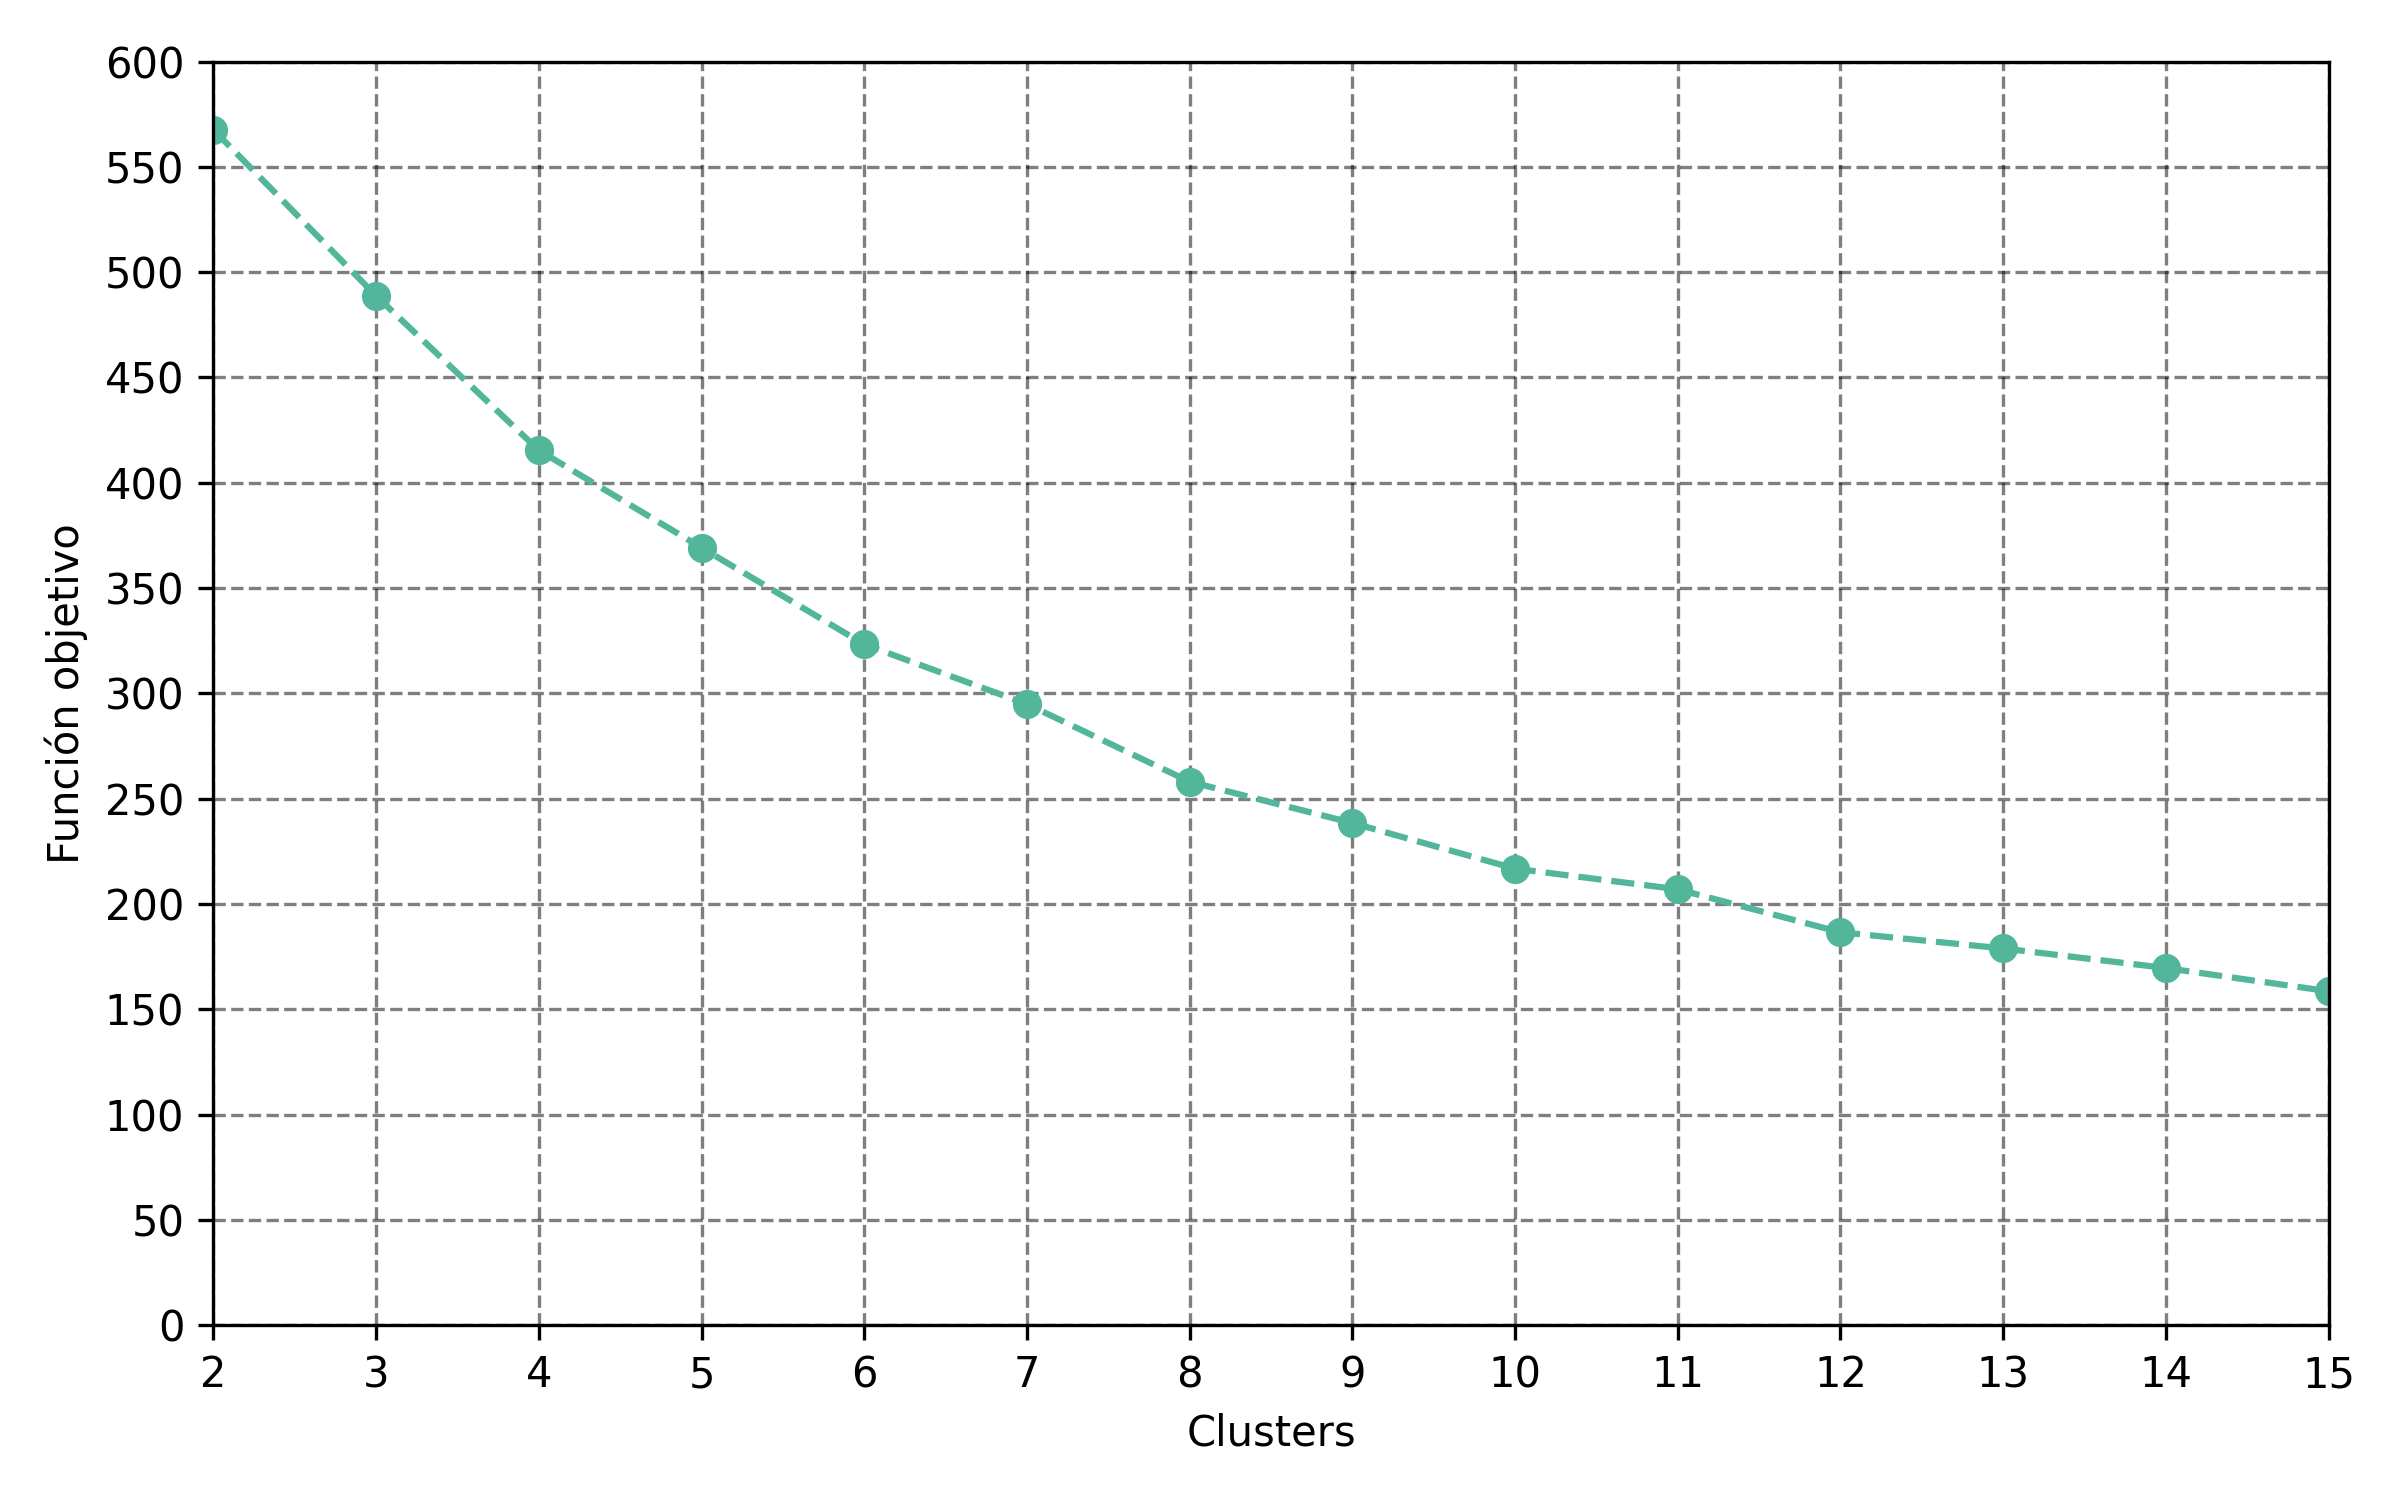
\includegraphics[width=12cm]{Graphics/Problema_03/train_scores.png}
    \caption{Valor de la función objetivo para los datos de entrenamiento.}
    \label{fig:problema_03_train_scores}
\end{figure}